% 超周边碰撞（UPC）—— TikZ 实现
% 按 ir/sketch5_upc.ir.yaml：纯线条无渐变，TikZ 是合适后端
\documentclass[border=0pt]{standalone}
\usepackage{tikz}
\usetikzlibrary{arrows.meta,decorations.pathmorphing,calc}
\renewcommand{\familydefault}{\sfdefault}
\begin{document}
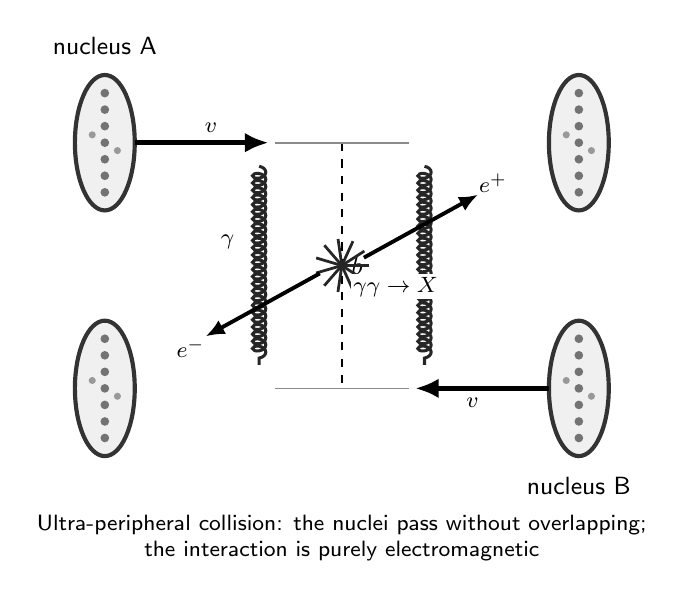
\begin{tikzpicture}[x=1cm,y=1cm, every node/.style={font=\small}]
  % 画布 400x190 pt = 14.06 x 6.68 cm

  % ⚠️ 不要写成 ellipse (0.38 and 0.86)：\def 宏展开时空格被吞，
  %    PGF 会看到 "0.38and 0.86" 并报 Unknown operator。
  %    核的半轴（纵向压扁，Lorentz 收缩）直接内联：0.38 x 0.86

  % ── E1 四个核 ──
  \foreach \x/\y in {4.02/4.90, 10.04/4.90, 4.02/1.78, 10.04/1.78}{
    \fill[black!6] (\x,\y) ellipse (0.38 and 0.86);
    \draw[line width=1.5pt, black!80] (\x,\y) ellipse (0.38 and 0.86);
    % 内部核子：竖排小球，暗示这是原子核而非空壳
    \foreach \i in {-3,...,3}{
      \fill[black!55] (\x, \y+\i*0.21) circle (0.055); }
    \fill[black!40] (\x-0.16, \y+0.10) circle (0.045);
    \fill[black!40] (\x+0.16, \y-0.10) circle (0.045); }
  \node[anchor=south] at (4.02,4.90+0.86+0.14) {nucleus A};
  \node[anchor=north] at (10.04,1.78-0.86-0.14) {nucleus B};

  % ── E2 速度箭头：A 向右、B 向左（相向）──
  % 核 A 向右：一个主箭头 + 一个虚线残影位置（表示"曾经在这里"）
  \draw[-{Latex[length=3.0mm,width=2.5mm]}, line width=2.0pt] (4.40,4.90) -- (6.10,4.90);
  % A 从左驶来 → 残影在【左】\n  \draw[dashed, line width=0.9pt, black!35] (3.18,4.90) ellipse (0.38 and 0.86);
  \node[above, font=\footnotesize] at (4.02+1.35,4.90) {$v$};
  % 核 B 向左：同理
  \draw[-{Latex[length=3.0mm,width=2.5mm]}, line width=2.0pt] (9.66,1.78) -- (7.96,1.78);
  % B 从右驶来 → 残影在【右】\n  \draw[dashed, line width=0.9pt, black!35] (10.88,1.78) ellipse (0.38 and 0.86);
  \node[below, font=\footnotesize] at (10.04-1.35,1.78) {$v$};

  % ── E3 碰撞参数 b ──

  \draw[dashed, line width=0.9pt] (7.03,4.90) -- (7.03,1.78);
  \draw[line width=0.6pt, black!45] (7.03-0.85,4.90) -- (7.03+0.85,4.90);
  \draw[line width=0.6pt, black!45] (7.03-0.85,1.78) -- (7.03+0.85,1.78);
  \node[right, font=\small] at (7.03,4.90*0.5+1.78*0.5) {$b$};

  % ── E4 光子交换线（两核之间）──
  \foreach \dx in {-1.05, 1.05}{
    \draw[decorate, decoration={coil, aspect=0.62, segment length=2.6pt,
          amplitude=2.4pt}, line width=1.1pt, black!85]
      (7.03+\dx,4.90-0.30) -- (7.03+\dx,1.78+0.30); }
  \node[font=\footnotesize] at (7.03-1.45,3.34+0.30) {$\gamma$};

  % ── E5 相互作用顶点 ──
  \coordinate (V) at (7.03,4.90*0.5+1.78*0.5);
  \foreach \a in {0,32.7,...,359}{
    \draw[line width=1.0pt, black!85] (V) -- ++(\a:0.34); }
  \node[below right=3pt, font=\footnotesize, fill=white, inner sep=1pt] at (V) {$\gamma\gamma\to X$};

  % ── E6 末态粒子（背对背）──
  % ★ 两体末态【背对背】：e+ 朝右上，e- 朝左下（动量守恒）
  \draw[-{Latex[length=2.4mm,width=2.0mm]}, line width=1.4pt]
    (V) ++(0.28,0.10) -- ++(1.45,0.80);
  \node[font=\footnotesize] at ($(V)+(1.92,1.05)$) {$e^+$};
  \draw[-{Latex[length=2.4mm,width=2.0mm]}, line width=1.4pt]
    (V) ++(-0.28,-0.10) -- ++(-1.45,-0.80);
  \node[font=\footnotesize] at ($(V)+(-1.92,-1.05)$) {$e^-$};

  % ── E7 说明 ──
  \node[anchor=north, font=\footnotesize, align=center] at (7.03,0.30)
    {Ultra-peripheral collision: the nuclei pass without overlapping;\\
     the interaction is purely electromagnetic};
\end{tikzpicture}
\end{document}
